% Document Type: LaTeX
% Master File: user-guide.tex
\chapter{A Brief Tour of PVS}
\label{system-tutorial}

In this section we introduce the system by developing a theory and doing a
simple proof.  This will introduce the most useful commands and provide a
glimpse into the normal usage of PVS.  You will get the most out of this
section if you are sitting in front of a terminal with PVS
installed.\footnote{If you don't have it installed, see the instructions
at \url{http://pvs.csl.sri.com}}.  In the following we assume some
familiarity with \unix\ and Emacs.  If you are unfamiliar with Emacs
you may want to look at the introduction in Appendix~\ref{emacs-intro} on
page~\pageref{emacs-intro}.

Start by going to a \unix\ shell and creating a working directory (using
\texttt{mkdir}). Next, change (\texttt{cd}) to this working directory and
start up PVS by typing \texttt{pvs}.\index{pvs@\texttt{pvs}}\footnote{You
may need to include a pathname, depending on where and how PVS is
installed.} This command executes a shell script which runs Emacs, loads
the necessary PVS Emacs extensions, and starts the PVS lisp image as a
subprocess.  See Chapter~\ref{customization} on
page~\pageref{customization} for further details on the \texttt{pvs}
command and its parameters.  After a few moments, you should see the
welcome screen\index{welcome screen} indicating the version of PVS being
run, the current directory, and instructions for getting help.  You may be
asked whether you want to create a new context in the directory; answer
\texttt{yes} unless it is the wrong directory or you don't have write
permission there, in which case you should answer \texttt{no} and provide
an alternative directory when prompted.  When you are ready to exit PVS,
type the key sequence \key{C-x C-c}.

In the following, PVS Emacs commands are given first in their long form,
followed by an alternative abbreviation and/or key binding in parentheses.
For example, the command for proving in PVS is given as \ecmd{prove}
(\ecmd{pr}, \key{C-c p}).  This command can be entered by holding down the
\texttt{Meta} key,\footnote{Most keyboards provide a \texttt{Meta}
key\index{Meta key@\texttt{Meta} key} (hence the \texttt{M-} prefix).  On
the \sun 4, this key is labeled $\Diamond$;\index{<> key@$\Diamond$ key}
IBM style keyboards tend to use the \texttt{Alt} key.\index{Alt
key@\texttt{Alt} key} The \texttt{Meta} key is like the shift key---to use
it simply hold the \texttt{Meta} key down while typing another key.  If
your keyboard does not have a \texttt{Meta} key, you can press the
\texttt{Escape} key for the same effect. Note that the \texttt{Escape} key
does not act as a shift, but is pressed and released before the command,
e.g. \texttt{Escape} followed by \texttt{x} followed by \texttt{pr}.} then
pressing \texttt{x}. Release the \texttt{Meta} key, then type
\texttt{prove} (or \texttt{pr}) and press the \texttt{Return} key.
Alternatively, hold the \texttt{Control} key down while typing a
\texttt{c}, then let go and type a \texttt{p}.  The \texttt{Return} key
does not need to be pressed when giving the key binding form.  In PVS all
commands and abbreviations are invoked by first typing a \texttt{M-x};
everything else is a key-binding.  In later sections we will refer to
commands by their long form name, without the \texttt{M-x} prefix.  Some
of the commands prompt for an argument and specify a default; if the
default is the desired one, you can simply type the \texttt{Return} key.

To begin, type \iecmd{pvs-help} (\texttt{C-c h}) for an overview of the
commands available in PVS, and use \texttt{C-v} and \texttt{M-v} to browse
the help file and get a feel for the commands provided by PVS.  Type
\texttt{q} to exit the help buffer.  If you are running Emacs under X
windows, you should see a menu bar across the top of the
window, including a \texttt{PVS} entry.  If you move the mouse cursor over
this entry, and press the left mouse button, a menu will be displayed that
also shows all the PVS commands (including the help commands).  This menu
may also be used to invoke the
commands, though most users prefer to learn the keyboard commands as this
is generally faster.  When discussing the PVS commands we will not mention
the PVS menu, but you should be aware that all of the PVS Emacs commands
are available as menu entries.

\section{Creating the Specification}

Now let's develop a small specification.  Figure~\ref{sum-screen} shows
a specification for summation of the first $n$ natural numbers, as it
appears in Emacs.  The \texttt{sum} specification is in the top window,
and a proof is in progress in the bottom.  The mode line indicates that
PVS is ready for a command.

\begin{figure}
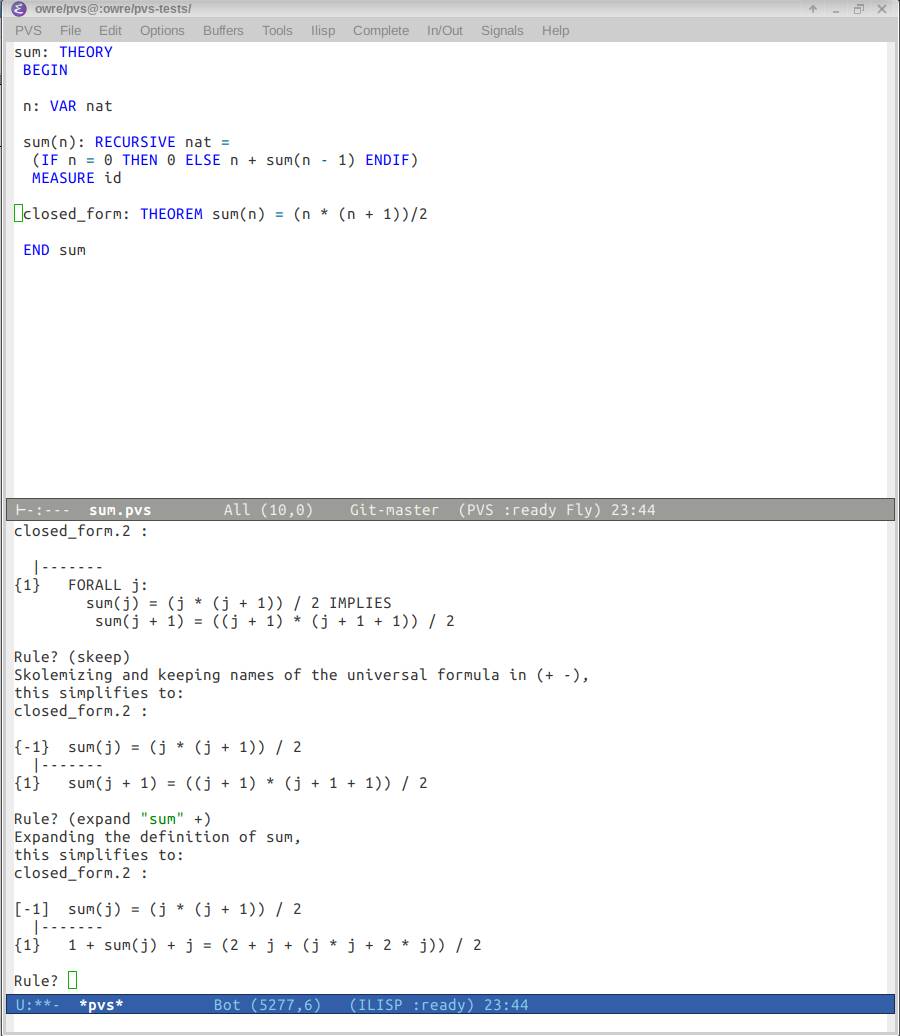
\includegraphics[width=\textwidth]{pvs-screen1.png}
\caption{The \texttt{sum} Specification in Emacs}\label{sum-screen}
\end{figure}

This simple theory has no parameters and contains three declarations.  The
first declares \texttt{n} to be a variable of type \texttt{nat}, the
built-in type of natural numbers.  The next declaration is a recursive
definition of the function \texttt{sum(n)} whose value is the sum of the
first \texttt{n} natural numbers.  Associated with this definition is a
\emph{measure} function, following the \texttt{MEASURE} keyword, which is
explained below.  The final declaration is a formula which gives the
closed form of the sum.

The \texttt{sum} theory may be introduced to the system in a number of
ways, all of which create a file with a \texttt{.pvs}
extension.\footnote{The file does not have to be named \texttt{sum.pvs}, it
simply needs the \texttt{.pvs} extension.}  The most common ways are:
\begin{enumerate}

\item Simply use \texttt{M-x find-file} (\key{C-x C-f}), or \texttt{M-x
find-pvs-file} (\ecmd{ff}, \key{C-c C-f}), provide \texttt{sum.pvs} for
the file name and type in the specification.\footnote{If there is already
a file called \texttt{sum.pvs} in the current context, this will load that
file.}

\item Use the \texttt{M-x new-pvs-file} command (\ecmd{nf}) to create a
new PVS file, and type \texttt{sum} when prompted for a file name.  Then
simply type the specification into the buffer (a basic template will be provided). 

\item Since the file is included in the distribution in the
\texttt{Examples} subdirectory of the main PVS directory, it can be
imported with the \texttt{M-x import-pvs-file} command (\ecmd{imf}).  Use
the \ecmd{whereis-pvs} command to find the path of the main PVS directory.

\item Finally, any external means of introducing a file with extension
\texttt{.pvs} into the current directory will make it available to the
system; for example, going to a \unix\ window and using \texttt{vi} to
type it in, or \texttt{cp} to copy it from the \texttt{Examples}
subdirectory.

\end{enumerate}

\section{Parsing and Typechecking}

Once the \texttt{sum} specification is displayed in the current buffer, it
can be parsed with the \iecmd{parse} (\ecmd{pa}) command, which checks the
syntactic consistency of the specification and creates the internal
abstract representation for the theory described by the specification.  If
the system finds an error during parsing, an error window will pop up with
an error message, and the cursor will be placed in the vicinity of the
error.  If you didn't get an error, introduce one (say by misspelling the
\texttt{VAR} keyword), then move the cursor somewhere else and parse the
file again---note that the buffer is automatically saved.  Fix the error
and parse once more.  In practice, the parse command is rarely used, as
the system automatically parses the specification when it needs to.

\index{typecheck|(}

The next step is to typecheck the file by typing \iecmd{typecheck}
(\iecmd{tc}, \key{C-c C-t}), which checks for semantic errors, such as
undeclared names and ambiguous types.  After \texttt{sum} has been
typechecked, a message is displayed in the minibuffer indicating that two
\tccs\index{TCCs@\tccs|(} were generated.  These \tccs\ represent
\emph{proof obligations}\index{proof obligations} that must be discharged
before the \texttt{sum} theory can be considered typechecked.  The proofs
of the \tccs\ may be postponed indefinitely, though in general it is a
good idea to view \tccs\ to convince yourself that they are provable
before moving on to other proofs in your specification.  \tccs\ can be
viewed using the \iecmd{show-tccs} (\iecmd{tccs}, \key{C-c C-q s})
command, the results of which are shown in Figure~\ref{sum-tccs} below.

\pvstheory{sum-tccs}{\tccs\ for Theory \texttt{sum}}{sum-tccs}

The first \tcc\ is due to the fact that \texttt{sum} takes an argument of
type \texttt{nat}, but the type of the argument in the recursive call to
\texttt{sum} is integer, since \texttt{nat} is not closed under subtraction.
Note that the \tcc\ includes the condition \texttt{NOT n = 0}, which holds
in the branch of the \texttt{IF-THEN-ELSE} in which the expression
\texttt{n - 1} occurs.

The second \tcc\ is needed to ensure that the function \texttt{sum} is
total, \ie\ terminates.  PVS does not directly support partial functions,
although its powerful subtyping mechanism allows PVS to express many
operations that are traditionally regarded as partial.  The measure
function is used to show that recursive definitions are total by requiring
the measure to decrease with each recursive call.

These \tccs\ are trivial, and in fact can be discharged automatically by
using the \ecmd{typecheck-prove} (\ecmd{tcp}) command, which attempts to
prove all \tccs\ that have been generated.  (Try it.)
\index{TCCs@\tccs|)}\index{typecheck|)}

\section{Proving}

We are now ready to try to prove the main theorem.  Place the cursor on
the line containing the \texttt{closed\_form} theorem, and type
\iecmd{prove} (\iecmd{pr} or \key{C-c p}).  A new buffer will pop up, the
formula will be displayed, and the cursor will appear at the
\texttt{Rule?}  prompt, indicating that the prover is ready to accept
input.  The commands needed to prove this theorem constitute only a very
small subset of the commands available to the prover.  In fact, for this
proof all that is actually needed is the single command
\texttt{(induct-and-simplify "n")}, which is a more powerful strategy.
For more information on these and other prover commands consult the prover
guide~\cite{PVS:prover}.

First, notice the display, which consists of a single formula (labeled
\texttt{\{1\}}) under a dashed line.  This is a
\emph{sequent}\index{sequent}; formulas above the dashed lines are called
\emph{antecedents}\index{antecedent} and those below are called
\emph{consequents}\index{consequent}.  The interpretation of a sequent is
that the conjunction of the antecedents implies the disjunction of the
consequents.  Either or both of the antecedents and consequents may be
empty.  An empty antecedent is equivalent to \texttt{true}, and an empty
consequent is equivalent to \texttt{false}, so if both are empty the
sequent is \texttt{false}.  Every proof in PVS starts with a single
consequent.

The basic objective of the proof is to generate a \emph{proof
tree}\index{proof tree} of sequents in which all of the leaves are
trivially true.  The nodes of the proof tree are sequents, and while in
the prover you will always be looking at an unproved leaf of the tree,
called the \emph{current} sequent.\index{current sequent} The
\emph{current} branch\index{current branch} of a proof is the branch
leading back to the root from the current sequent.  When a given branch is
complete (\ie\ ends in a proved leaf), the prover automatically moves on
to the next unproved branch, or, if there are no more unproven branches,
notifies you that the proof is complete.

Now on to the proof.  We will prove this formula by induction on
\texttt{n}.  To do this, type \texttt{(induct "n")}\index{prover
commands!induct@\texttt{induct}}.\footnote{PVS expressions are
case-sensitive, and must be put in double quotes when they appear as
arguments in prover commands.} This is not an Emacs command, rather it
is typed directly at the prompt, including the parentheses.  As indicated,
two subgoals are generated; the one displayed is the base case, where
\texttt{n} is \texttt{0}.  To see the inductive step, type
\texttt{(postpone)}\index{prover commands!postpone@\texttt{postpone}},
which postpones the current subgoal and moves on to the next unproved one.
Type \texttt{(postpone)} a second time to cycle back to the original
subgoal (labeled \texttt{closed\_form.1}).

Three extremely useful Emacs key bindings to know here are \key{M-p},
\key{M-n}, and \key{M-s}.  \key{M-p} gets the last input typed to the
prover; further uses of \key{M-p} cycle back in the input history.
\key{M-n} works in the opposite direction.  To use \key{M-s}, type the
beginning of a command that was previously input, and type \key{M-s}.
This will get the previous input that matches the partial input; further
uses of \key{M-s} will find earlier matches.  Try these key bindings out;
they are easier to use than to explain.  Thus to type the second postpone
command above, you can either type \key{M-p} or type \texttt{(po} followed
by \key{M-s}.  Section~\ref{prover-emacs} on page~\pageref{prover-emacs}
describes further useful shortcut commands for the prover.

To prove the base case, we need to expand the definition of \texttt{sum},
which is done by typing \texttt{(expand "sum")}\index{prover
commands!expand@\texttt{expand}}.  After expanding the definition of
\texttt{sum}, we issue the \texttt{(assert)}\index{prover
commands!assert@\texttt{assert}} command, which applies the decision
procedures of the prover to simplify the consequent to \texttt{TRUE},
completing the proof of this subgoal.  The prover then automatically moves
on to the next subgoal, which is the inductive step.

The first thing to do here is to eliminate the \texttt{FORALL} quantifier.
This can most easily be done with the \texttt{skolem!}\ \index{prover
commands!skolem@\texttt{skolem"!}}  command\footnote{The exclamation point
differentiates this command from the \texttt{skolem} command, where you
provide the new constant names.}, which provides new constants for the
bound variables.  To invoke this command type \texttt{(skolem!)} at the
prompt.  The resulting formula may be simplified by typing
\texttt{(flatten)}\index{prover commands!flatten@\texttt{flatten}}, which
will break up the consequent into a new antecedent and consequent.  The
obvious thing to do now is to expand the definition of \texttt{sum} in the
consequent.  This again is done with the \texttt{expand} command, but this
time we want to control where it is expanded, as expanding it in the
antecedent will not help.  So we type \texttt{(expand "sum" +)},
indicating that we want to expand \texttt{sum} in the
consequent.\footnote{We could also have specified the exact formula number
(here \texttt{1}), but including formula numbers in a proof tends to make
it less robust in the face of changes.  There is more discussion of this
in the prover guide~\cite{PVS:prover}.}

The final step is to invoke the PVS decision procedures, which can
automatically decide certain fragments of arithmetic.  This is done by
typing \texttt{(assert)}. The \texttt{assert}\index{prover
commands!assert@\texttt{assert}} command actually does a lot more than
decide arithmetical formulas, performing three basic tasks:
\begin{itemize}\def\itemsep{0in}
\item It tries to prove the subgoal using the decision procedures.

\item It stores the subgoal information in an underlying database,
allowing automatic use to be made of it later.

\item It simplifies the subgoal by rewriting (if any auto-rewrites have
been given) and by using the underlying decision procedures.
\end{itemize}
These arithmetic and equality procedures are the main workhorses of most
PVS proofs.

The proof is now complete, and is saved in the \texttt{sum.prf} file.  The
buffer from which the \cmd{prove} command was issued is then redisplayed
if necessary, and the cursor is placed on the formula that was just
proved.  The entire proof transcript is shown below.  Yours may be
slightly different, depending on your window size and the timings involved.

{\smaller\smaller
\begin{alltt}
  closed_form :  

    |-------
  \{1\}   FORALL (n: nat): sum(n) = n * (n + 1) / 2

  Rule? (induct "n")
  Inducting on n on formula 1,
  this yields  2 subgoals: 
  closed_form.1 :  

    |-------
  \{1\}   sum(0) = 0 * (0 + 1) / 2

  Rule? (postpone)
  Postponing closed_form.1.

  closed_form.2 :  

    |-------
  \{1\}   FORALL (j: nat):
          sum(j) = j * (j + 1) / 2 IMPLIES sum(j + 1) = (j + 1) * (j + 1 + 1) / 2

  Rule? (postpone)
  Postponing closed_form.2.

  closed_form.1 :  

    |-------
  \{1\}   sum(0) = 0 * (0 + 1) / 2

  Rule? (expand "sum")
  Expanding the definition of sum,
  this simplifies to: 
  closed_form.1 :  

    |-------
  \{1\}   0 = 0 / 2

  Rule? (assert)
  Simplifying, rewriting, and recording with decision procedures,

  This completes the proof of closed_form.1.

  closed_form.2 :  

    |-------
  \{1\}   FORALL (j: nat):
          sum(j) = j * (j + 1) / 2 IMPLIES sum(j + 1) = (j + 1) * (j + 1 + 1) / 2

  Rule? (skolem!)
  Skolemizing,
  this simplifies to: 
  closed_form.2 :  

    |-------
  \{1\}   sum(j!1) = j!1 * (j!1 + 1) / 2 IMPLIES
         sum(j!1 + 1) = (j!1 + 1) * (j!1 + 1 + 1) / 2

  Rule? (flatten)
  Applying disjunctive simplification to flatten sequent,
  this simplifies to: 
  closed_form.2 :  

  \{-1\}  sum(j!1) = j!1 * (j!1 + 1) / 2
    |-------
  \{1\}   sum(j!1 + 1) = (j!1 + 1) * (j!1 + 1 + 1) / 2

  Rule? (expand "sum" +)
  Expanding the definition of sum,
  this simplifies to: 
  closed_form.2 :  

  [-1]  sum(j!1) = j!1 * (j!1 + 1) / 2
    |-------
  \{1\}   1 + sum(j!1) + j!1 = (2 + j!1 + (j!1 * j!1 + 2 * j!1)) / 2

  Rule? (assert)
  Simplifying, rewriting, and recording with decision procedures,

  This completes the proof of closed_form.2.

  Q.E.D.


  Run time  = 0.81 secs.
  Real time = 223.01 secs.

\end{alltt}}

A brief version of the just completed proof can be generated by the command
command \iecmd{show-last-proof}.

\section{Status}

Now type \iecmd{status-proof-theory} (\iecmd{spt}) and you will see a
buffer that displays the three formulas in \texttt{sum}, along with an
indication of their proof status.  This command is useful to see which
formulas and \tccs\ still require proofs.  Another useful command is
\iecmd{status-proofchain} (\ecmd{spc}), which analyzes a given proof to
determine its dependencies.  To use this, go to the \texttt{sum.pvs}
buffer, place the cursor on the \texttt{closed\_form} theorem, and enter
the command.  A buffer will pop up indicating that the proof is
complete, and that it depends on the \tccs\ and the \texttt{nat\_induction}
axiom, as well as some definitions and \tccs\ provided by the prelude.

\section{Generating \LaTeX}

In order to try out this section, you must have access to \LaTeX\
\index{LaTeX@\LaTeX} and a \TeX\ previewer such as
\texttt{xdvi}\index{xdvi}.

Type \iecmd{latex-theory-view} (\iecmd{ltv}).  You will be prompted for
the theory name to which you should type \texttt{sum}, or just
\texttt{Return} if \texttt{sum} is the default.  You will then be prompted
for the \TeX\ previewer name.  Either the previewer must be in your path,
or the entire pathname must be given.  This information will only be
prompted for once per session, after which PVS assumes that you want to
use the same previewer.  You can set the previewer automatically,
by adding the following line to your \texttt{\char'176/.pvsemacs} file.
{\small
\begin{alltt}
\hspace*{2em}  (setq pvs-latex-viewer "\textit{previewer}")
\end{alltt}}

\begin{figure}[ht]
\begin{center}
\begin{boxedminipage}{\textwidth}
{\small\small\input{sum-nosub}}
\end{boxedminipage}
\end{center}
\caption{Theory \texttt{sum} with default translations}\label{sum-plain}
\end{figure}

After a few moments the previewer will pop up displaying the \texttt{sum}
theory, as shown in Figure~\ref{sum-plain}.  Note that \texttt{*} has been
translated as $\times$ and \texttt{LAMBDA} as $\lambda$.  These and other
translations are built into PVS; you may also specify translations for
keywords and identifiers by providing a substitution file named
\texttt{pvs-tex.sub}, that contains commands to customize the \LaTeX\
output.  For example, if the substitution file contains the two lines
{\small\small
\begin{alltt}
    THEORY key 7 \verb|{\large\textbf{\textrm{Theory}}}|
    sum    1   2 \verb|{\sum_{i = 0}^{#1} i}|
\end{alltt}}
\noindent the output will look like Figure~\ref{sum-sub}.  See
Section~\ref{latex-output} on page~\pageref{latex-output} for more
details.

\begin{figure}[t]
\begin{boxedminipage}{\textwidth}
{\small\small% The following substitutions are from the file:
%   /home/owre/pvs.git/pvs-tex.sub
\def\munderscoretimestwofn#1#2{{#1 \times #2}}% How to print function m_times with arity (2)
\def\fmunderscoretimestwofn#1#2{{#1 \times #2}}% How to print function fm_times with arity (2)
\def\sigmaunderscoretimestwofn#1#2{{#1 \times #2}}% How to print function sigma_times with arity (2)
\def\generatedunderscoresubsetunderscorealgebraonefn#1{{{\cal A}(#1)}}% How to print function generated_subset_algebra with arity (1)
\def\generatedunderscoresigmaunderscorealgebraonefn#1{{{\cal S}(#1)}}% How to print function generated_sigma_algebra with arity (1)
\def\aeunderscoredecreasingotheronefn#1{{\pvsid{decreasing?}(#1)~\mbox{\it a.e.}}}% How to print function ae_decreasing? with arity (1)
\def\aeunderscoreincreasingotheronefn#1{{\pvsid{increasing?}(#1)~\mbox{\it a.e.}}}% How to print function ae_increasing? with arity (1)
\def\aeunderscoreconvergenceothertwofn#1#2{{#1 \longrightarrow #2~\mbox{\it a.e.}}}% How to print function ae_convergence? with arity (2)
\def\aeunderscoreeqothertwofn#1#2{{#1 = #2~\mbox{\it a.e.}}}% How to print function ae_eq? with arity (2)
\def\aeunderscoreleothertwofn#1#2{{#1 \leq #2~\mbox{\it a.e.}}}% How to print function ae_le? with arity (2)
\def\aeunderscoreposotheronefn#1{{#1> 0~\mbox{\it a.e.}}}% How to print function ae_pos? with arity (1)
\def\aeunderscorenonnegotheronefn#1{{#1 \geq 0~\mbox{\it a.e.}}}% How to print function ae_nonneg? with arity (1)
\def\aeunderscorezerootheronefn#1{{#1 = 0~\mbox{\it a.e.}}}% How to print function ae_0? with arity (1)
\def\xunderscorelttwofn#1#2{{#1 < #2}}% How to print function x_lt with arity (2)
\def\xunderscoreletwofn#1#2{{#1 \leq #2}}% How to print function x_le with arity (2)
\def\xunderscoreeqtwofn#1#2{{#1 = #2}}% How to print function x_eq with arity (2)
\def\xunderscoretimestwofn#1#2{{#1 \times #2}}% How to print function x_times with arity (2)
\def\xunderscoreaddtwofn#1#2{{#1 + #2}}% How to print function x_add with arity (2)
\def\xunderscorelimitonefn#1{{\pvsid{limit}(#1)}}% How to print function x_limit with arity (1)
\def\xunderscoresumonefn#1{{\sum #1}}% How to print function x_sum with arity (1)
\def\xunderscoresigmathreefn#1#2#3{{\sum_{#1}^{#2} #3}}% How to print function x_sigma with arity (3)
\def\xunderscoresuponefn#1{{\pvsid{sup}(#1)}}% How to print function x_sup with arity (1)
\def\xunderscoreinfonefn#1{{\pvsid{inf}(#1)}}% How to print function x_inf with arity (1)
\def\pointwiseunderscoreconvergesunderscoredowntoothertwofn#1#2{{#1 \searrow #2}}% How to print function pointwise_converges_downto? with arity (2)
\def\pointwiseunderscoreconvergesunderscoreuptoothertwofn#1#2{{#1 \nearrow #2}}% How to print function pointwise_converges_upto? with arity (2)
\def\pointwiseunderscoreconvergenceothertwofn#1#2{{#1 \longrightarrow #2}}% How to print function pointwise_convergence? with arity (2)
\def\convergesunderscoredowntoothertwofn#1#2{{#1 \searrow #2}}% How to print function converges_downto? with arity (2)
\def\convergesunderscoreuptoothertwofn#1#2{{#1 \nearrow #2}}% How to print function converges_upto? with arity (2)
\def\convergenceothertwofn#1#2{{#1 \longrightarrow #2}}% How to print function convergence? with arity (2)
\def\convergencetwofn#1#2{{#1 \longrightarrow #2}}% How to print function convergence with arity (2)
\def\crossunderscoreproducttwofn#1#2{{#1 \times #2}}% How to print function cross_product with arity (2)
\def\conjugateonefn#1{{\overline{#1}}}% How to print function conjugate with arity (1)
\def\cunderscoredivtwofn#1#2{{#1/#2}}% How to print function c_div with arity (2)
\def\cunderscoremultwofn#1#2{{#1\times#2}}% How to print function c_mul with arity (2)
\def\cunderscoresubtwofn#1#2{{#1-#2}}% How to print function c_sub with arity (2)
\def\cunderscorenegonefn#1{{-#1}}% How to print function c_neg with arity (1)
\def\cunderscoreaddtwofn#1#2{{#1+#2}}% How to print function c_add with arity (2)
\def\Imonefn#1{{\Im(#1)}}% How to print function Im with arity (1)
\def\Reonefn#1{{\Re(#1)}}% How to print function Re with arity (1)
\def\Etwofn#1#2{{\mathbb{E}(#1~|~#2)}}% How to print function E with arity (2)
\def\Eonefn#1{{\mathbb{E}(#1)}}% How to print function E with arity (1)
\def\Ptwofn#1#2{{\mathbb{P}(#1~|~#2)}}% How to print function P with arity (2)
\def\Ponefn#1{{\mathbb{P}(#1)}}% How to print function P with arity (1)
\def\xtwofn#1#2{{#1\times#2}}% How to print function x with arity (2)
\def\asttwofn#1#2{{#1\ast#2}}% How to print function ast with arity (2)
\def\minusonefn#1{{{#1}^{-}}}% How to print function minus with arity (1)
\def\plusonefn#1{{{#1}^{+}}}% How to print function plus with arity (1)
\def\astonefn#1{{{#1}^{\ast}}}% How to print function ast with arity (1)
\def\dottwofn#1#2{{#1\bullet#2}}% How to print function dot with arity (2)
\def\integralthreefn#1#2#3{{\int_{#1}^{#2} #3}}% How to print function integral with arity (3)
\def\integraltwofn#1#2{{\int_{#1} #2}}% How to print function integral with arity (2)
\def\integralonefn#1{{\int#1}}% How to print function integral with arity (1)
\def\normonefn#1{{\left||{#1}\right||}}% How to print function norm with arity (1)
\def\phionefn#1{{\pvssubscript{\phi}{#1}}}% How to print function phi with arity (1)
\def\infunderscoreclosedonefn#1{{\left(-\infty,~#1\right]}}% How to print function inf_closed with arity (1)
\def\closedunderscoreinfonefn#1{{\left[#1,~\infty\right)}}% How to print function closed_inf with arity (1)
\def\infunderscoreopenonefn#1{(-\infty,~#1)}% How to print function inf_open with arity (1)
\def\openunderscoreinfonefn#1{(#1,~\infty)}% How to print function open_inf with arity (1)
\def\closedtwofn#1#2{{\left[#1,~#2\right]}}% How to print function closed with arity (2)
\def\opentwofn#1#2{(#1,~#2)}% How to print function open with arity (2)
\def\sigmathreefn#1#2#3{{\sum_{#1}^{#2} #3}}% How to print function sigma with arity (3)
\def\sigmatwofn#1#2{{\sum_{#1} {#2}}}% How to print function sigma with arity (2)
\def\ceilingonefn#1{{\lceil{#1}\rceil}}% How to print function ceiling with arity (1)
\def\flooronefn#1{{\lfloor{#1}\rfloor}}% How to print function floor with arity (1)
\def\absonefn#1{{\left|{#1}\right|}}% How to print function abs with arity (1)
\def\roottwofn#1#2{{\sqrt[#2]{#1}}}% How to print function root with arity (2)
\def\sqrtonefn#1{{\sqrt{#1}}}% How to print function sqrt with arity (1)
\def\sqonefn#1{{\pvssuperscript{#1}{2}}}% How to print function sq with arity (1)
\def\expttwofn#1#2{{\pvssuperscript{#1}{#2}}}% How to print function expt with arity (2)
\def\opcarettwofn#1#2{{\pvssuperscript{#1}{#2}}}% How to print function ^ with arity (2)
\def\indexedunderscoresetsotherIIntersectiononefn#1{{\bigcap #1}}% How to print function indexed_sets.IIntersection with arity (1)
\def\indexedunderscoresetsotherIUniononefn#1{{\bigcup #1}}% How to print function indexed_sets.IUnion with arity (1)
\def\setsotherIntersectiononefn#1{{\bigcap #1}}% How to print function sets.Intersection with arity (1)
\def\setsotherUniononefn#1{{\bigcup #1}}% How to print function sets.Union with arity (1)
\def\setsotherremovetwofn#1#2{{(#2 \setminus \{#1\})}}% How to print function sets.remove with arity (2)
\def\setsotheraddtwofn#1#2{{(#2 \cup \{#1\})}}% How to print function sets.add with arity (2)
\def\setsotherdifferencetwofn#1#2{{(#1 \setminus #2)}}% How to print function sets.difference with arity (2)
\def\setsothercomplementonefn#1{{\overline{#1}}}% How to print function sets.complement with arity (1)
\def\setsotherintersectiontwofn#1#2{{(#1 \cap #2)}}% How to print function sets.intersection with arity (2)
\def\setsotheruniontwofn#1#2{{(#1 \cup #2)}}% How to print function sets.union with arity (2)
\def\setsotherstrictunderscoresubsetothertwofn#1#2{{(#1 \subset #2)}}% How to print function sets.strict_subset? with arity (2)
\def\setsothersubsetothertwofn#1#2{{(#1 \subseteq #2)}}% How to print function sets.subset? with arity (2)
\def\setsothermembertwofn#1#2{{(#1 \in #2)}}% How to print function sets.member with arity (2)
\def\opohtwofn#1#2{{#1\circ#2}}% How to print function O with arity (2)
\def\opdividetwofn#1#2{{\frac{#1}{#2}}}% How to print function / with arity (2)
\def\optimestwofn#1#2{{#1\times#2}}% How to print function * with arity (2)
\def\opdifferenceonefn#1{{-#1}}% How to print function - with arity (1)
\def\opdifferencetwofn#1#2{{#1-#2}}% How to print function - with arity (2)
\def\opplustwofn#1#2{{#1+#2}}% How to print function + with arity (2)
% The following substitutions are from the file:
%   /home/owre/pvs.git/doc/wift95/pvs-tex.sub
\def\sumonefn#1{{\sum_{i = 0}^{#1} i}}% How to print function sum with arity (1)
\begin{alltt}
\pvsid{sum}: \({\large\bf Theory}\)
 \pvskey{BEGIN}

  \(n\): \pvskey{VAR} \(\mathbb{N}\)\vspace*{\pvsdeclspacing}

  \(\sumonefn{n}\): \pvskey{RECURSIVE} \(\mathbb{N}\) \pvskey{=} \pvsid{(}\pvskey{IF} \(n\) \(=\) \(0\) \pvskey{THEN} \(0\) \pvskey{ELSE} \(\opplustwofn{n}{\sumonefn{\opdifferencetwofn{n}{1}}}\) \pvskey{ENDIF}\pvsid{)}
     \pvskey{MEASURE} \pvsid{(}\(\lambda\) \(n\): \(n\)\pvsid{)}\vspace*{\pvsdeclspacing}

  \pvsid{closed\_form}: \pvskey{THEOREM} \(\sumonefn{n}\) \(=\) \(\opdividetwofn{\pvsid{(}\optimestwofn{n}{\pvsid{(}\opplustwofn{n}{1}\pvsid{)}}\pvsid{)}}{2}\)\vspace*{\pvsdeclspacing}

 \pvskey{END} \pvsid{sum}\end{alltt}
}
\end{boxedminipage}
\caption{Theory \texttt{sum} with additional translations}\label{sum-sub}
\end{figure}

\vspace*{1in}
